% Copyright Luke Olson 2009--2014
% This work is licensed under the Creative Commons
% Attribution-NonCommercial-NoDerivatives 4.0 International License. To view a
% copy of this license, visit http://creativecommons.org/licenses/by-nc-nd/4.0/.
%
\documentclass[10pt]{beamer}
%\documentclass[handout,10pt]{beamer}
%
\mode<presentation>
{
  \usetheme[secheader]{Boadilla}
  \usefonttheme[onlymath]{serif}
  \setbeamercovered{invisible}
  \usecolortheme{luke}
  %\setbeamercovered{transparent}
  %
}
\mode<handout>
{
  \usetheme[secheader]{Boadilla}
  \usefonttheme[onlymath]{serif}
  \setbeamercovered{invisible}
  \usecolortheme{luke2}
  %\setbeamercovered{transparent}
}
\usepackage{pgf,pgfarrows,pgfnodes,pgfautomata,pgfheaps,pgfshade}
\usepackage{pxfonts}
\usepackage{eulervm}
\usepackage{listings}
%\usepackage{pgfpages}
%\pgfpagesuselayout{2 on 1}[letterpaper]
%
%
%%%%%%%%%%%%%%%%%%%%%%%%%%%%%%%%%%%%%%%%%%%%%%%%%%%%%%%%%%%%%%%%%%%%%%%%


%
%
%
\newcommand{\vb}{{\bf{b}}}
\newcommand{\ve}{{\bf{e}}}
\newcommand{\vg}{{\bf{g}}}
\newcommand{\vp}{{\bf{p}}}
\newcommand{\vr}{{\bf{r}}}
\newcommand{\vu}{{\bf{u}}}
\newcommand{\vx}{{\bf{x}}}
\newcommand{\vz}{{\bf{z}}}
\newcommand{\vA}{{\bf{A}}}
\newcommand{\vU}{{\bf{U}}}
\newcommand{\mO}{{\mathcal{O}}}
\newcommand{\mF}{{\mathcal{F}}}
\definecolor{mygray}{rgb}{0.95,0.95,0.95}
\lstset{
        language=matlab,
        numbers=left, numberstyle=\tiny, stepnumber=1, numbersep=5pt,
        basicstyle=\color{black}\ttfamily\small,
        commentstyle=\color{green}\ttfamily,
        keywordstyle=\color{blue}\ttfamily,
        stringstyle=\color{red}\ttfamily,
        showstringspaces=false,
        backgroundcolor=\color{mygray},
        breaklines,
}

\author{L. Olson}
\institute[UIUC]
{Department of Computer Science\\
University of Illinois at Urbana-Champaign\\
\vspace{0.5cm}
}
%%%%%%%%%%%%%%%%%%%%%%%%%%%%%%%%%%%%%%%%%%%%%%%%%%%%%%%%%%%%%%%%%%%%%%%%
\pgfdeclareimage[height=0.5cm]{university-logo}{./figs/uiuclogo}
\logo{\pgfuseimage{university-logo}}
%%%%%%%%%%%%%%%%%%%%%%%%%%%%%%%%%%%%%%%%%%%%%%%%%%%%%%%%%%%%%%%%%%%%%%%%
\title[CS 357]{Lecture 13}
\subtitle{Rootfinding: Secant Method}
\date{October 8, 2009}

\begin{document}
% -------------------------------------------------
\begin{frame}
  \titlepage
\end{frame}
% -------------------------------------------------
%%%%%%%%%%%%%%%%%%%%%%%%%%%%%%%%%%%%%%%%%%%%%%%%%%%%%%%%%%%%%%%%%%%%%%%%
\begin{frame}
\frametitle{Convergence rate of a root finding iteration}
\begin{itemize}
  \item Let $e_n = x^* - x_n$ be the error.
  \item In general, a sequence is said to converge with rate $r$ if
    \begin{equation*}
      \lim_{k\rightarrow\infty} \frac{|e_{n+1}|}{|e_{n}|^{r}} = C
    \end{equation*}
\end{itemize}
\begin{block}{Special Cases:}
\begin{itemize}
  \item If $r=1$ and $C=1$, then the rate is \emph{sublinear}
  \item If $r=1$ and $C<1$, then the rate is \emph{linear}
  \item If $r>1$ (i.e. $r=1$ and $C=0$), then the rate is \emph{superlinear}
  \item If $r=2$ and $C>0$, then the rate is \emph{quadratic}
  \item If $r=3$ and $C>0$, then the rate is \emph{cubic}
\end{itemize}
\end{block}
\end{frame}
% -------------------------------------------------
%%%%%%%%%%%%%%%%%%%%%%%%%%%%%%%%%%%%%%%%%%%%%%%%%%%%%%%%%%%%%%%%%%%%%%%%
\begin{frame}[shrink]
\frametitle{Newton's Method: Convergence}
\begin{block}{Recall}
  Convergence of a method is said to be of order $r$ if there is a
constant $C>0$ such that
\begin{equation*}
  \lim_{k\rightarrow \infty} \frac{|e_{k+1}|}{|e_k|^r} = C
\end{equation*}
\end{block}
Newton's method is of order 2 (quadratic) when $f'(x_{*}) \ne 0$.
\bigskip
For $\xi$ between $x_k$ and $x_{*}$
\begin{equation*}
  f(x_{*}) = f(x_k) + (x_{*}-x_k)f'(x_k) + \frac{1}{2}(x_{*}-x_k)^2 f''(\xi) = 0
\end{equation*}
So
\begin{equation*}
  \frac{f(x_k)}{f'(x_k)} + x_{*}-x_k + (x_{*}-x_k)^2 \frac{f''(\xi)}{f'(x_k)} = 0
\end{equation*}
Then
\begin{equation*}
  \left(\frac{f(x_k)}{f'(x_k)} -x_k\right)+ x_{*} + (x_{*}-x_k)^2 \frac{f''(\xi)}{f'(x_k)} = 0
\end{equation*}
\begin{equation*}
  x_{*}-x_{k+1} + (x_{*}-x_k)^2 \frac{f''(\xi)}{f'(x_k)} = 0
\end{equation*}
Thus
\begin{equation*}
  \frac{\left|x_{*}-x_{k+1}\right|}{\left|x_{*}-x_k\right|^2}  = \left|\frac{f''(\xi)}{f'(x_k)}\right|
\end{equation*}
\end{frame}
%%%%%%%%%%%%%%%%%%%%%%%%%%%%%%%%%%%%%%%%%%%%%%%%%%%%%%%%%%%%%%%%%%%%%%%%
\begin{frame}
\frametitle{Secant Method}

\vspace{4ex}
\begin{center}
	\pgfimage[height=3cm]{./figs/secant}
\end{center}

Given two guesses $x_{k-1}$ and $x_k$, the next guess at the root
is where the line through $f(x_{k-1})$ and $f(x_k)$
crosses the $x$ axis.



% ------------
\end{frame}
%%%%%%%%%%%%%%%%%%%%%%%%%%%%%%%%%%%%%%%%%%%%%%%%%%%%%%%%%%%%%%%%%%%%%%%%
%%%%%%%%%%%%%%%%%%%%%%%%%%%%%%%%%%%%%%%%%%%%%%%%%%%%%%%%%%%%%%%%%%%%%%%%
\begin{frame}
\frametitle{Secant Method}

Given
\begin{align*}
    x_k     &= \mathrm{current\ guess\ at\ the\ root}\\
    x_{k-1} &= \mathrm{previous\ guess\ at\ the\ root}
\end{align*}

Approximate the first derivative with
\begin{equation*}
    f'(x_k) \approx \frac{f(x_k) - f(x_{k-1})}{x_k - x_{k-1}}
\end{equation*}

Substitute approximate $f'(x_k)$ into formula for Newton's method
\begin{equation*}
    x_{k+1} = x_k - \frac{f(x_k)}{f'(x_k)}
\end{equation*}
to get
\begin{equation*}
    x_{k+1} = x_k - f(x_k) \left[ \frac{x_k - x_{k-1}}{f(x_k) - f(x_{k-1})} \right]
\end{equation*}



% ------------
\end{frame}
%%%%%%%%%%%%%%%%%%%%%%%%%%%%%%%%%%%%%%%%%%%%%%%%%%%%%%%%%%%%%%%%%%%%%%%%
%%%%%%%%%%%%%%%%%%%%%%%%%%%%%%%%%%%%%%%%%%%%%%%%%%%%%%%%%%%%%%%%%%%%%%%%
\begin{frame}
\frametitle{Secant Method}

\vspace{3ex}
Two versions of this formula are (equivalent in exact math)
\begin{equation*}
    x_{k+1} = x_k - f(x_k) \left[ \frac{x_k - x_{k-1}}{f(x_k) - f(x_{k-1})} \right]  \tag{$\star$}
\end{equation*}
and
\begin{equation*}
    x_{k+1} = \frac{f(x_k) x_{k-1} - f(x_{k-1}) x_k}{f(x_k) - f(x_{k-1})}  \tag{$\star\star$}
\end{equation*}

Equation~($\star$) is better since it is of the form $x_{k+1} = x_k + \Delta$.
Even if $\Delta$ is inaccurate the change in the estimate of the
root will be small at convergence because $f(x_k)$ will also
be small.

Equation~($\star\star$) is susceptible to catastrophic cancellation:
\vspace{0.0cm}
\begin{itemize}
    \item   $f(x_k)\rightarrow f(x_{k-1})$ as convergence approaches,
            so cancellation error in denominator can be large.
    \item   $|f(x)|\rightarrow 0$ as convergence approaches,
            so underflow is possible
\end{itemize}



% ------------
\end{frame}
%%%%%%%%%%%%%%%%%%%%%%%%%%%%%%%%%%%%%%%%%%%%%%%%%%%%%%%%%%%%%%%%%%%%%%%%
%%%%%%%%%%%%%%%%%%%%%%%%%%%%%%%%%%%%%%%%%%%%%%%%%%%%%%%%%%%%%%%%%%%%%%%%
\begin{frame}[fragile]
\frametitle{Secant Algorithm}

\begin{lstlisting}[mathescape,caption=,label=algo:secant]
  initialize:  $x_1 = \ldots$, $x_2 = \ldots$                   
  for $k=2,3\ldots$                                           
    $x_{k+1} = x_k - f(x_k) (x_k - x_{k-1})/(f(x_k) - f(x_{k-1}) )$  
    if converged, stop       
  end
\end{lstlisting}





% ------------
\end{frame}
%%%%%%%%%%%%%%%%%%%%%%%%%%%%%%%%%%%%%%%%%%%%%%%%%%%%%%%%%%%%%%%%%%%%%%%%
%%%%%%%%%%%%%%%%%%%%%%%%%%%%%%%%%%%%%%%%%%%%%%%%%%%%%%%%%%%%%%%%%%%%%%%%
\begin{frame}
\frametitle{Secant Example}

Solve:
\begin{equation*}
    x - x^{1/3} - 2 = 0
\end{equation*}

\vspace{2ex}
\begin{center}
  \small
    \begin{tabular}{cccc}
       $k$ &   $x_{k-1}$  &    $x_k$   & $f(x_k)$                  \\ \hline
        0  &  4           & 3          & $-0.44224957$               \\
        1  &  3           & 3.51734262 & $-0.00345547$               \\
        2  &  3.51734262  & 3.52141665 & $0.00003163 $              \\
        3  &  3.52141665  & 3.52137970 & $-2.034\times 10^{-9}$  \\
        4  &  3.52137959  & 3.52137971 & $-1.332\times 10^{-15}$ \\
        5  &  3.52137971  & 3.52137971 &  0.0                      \\
        \end{tabular}
\end{center}

\vspace{4ex}

\textbf{Conclusions:}
\vspace{0.0cm}
\begin{itemize}
    \item   Converges almost as quickly as Newton's method ($r\approx
1.62$).
    \item   There is no need to compute $f'(x)$.
    \item   The algorithm is simple.
    \item   Two initial guesses are necessary
    \item   Iterations are not guaranteed to stay inside an ordinal bracket.
\end{itemize}




% ------------
\end{frame}
%%%%%%%%%%%%%%%%%%%%%%%%%%%%%%%%%%%%%%%%%%%%%%%%%%%%%%%%%%%%%%%%%%%%%%%%
%%%%%%%%%%%%%%%%%%%%%%%%%%%%%%%%%%%%%%%%%%%%%%%%%%%%%%%%%%%%%%%%%%%%%%%%
\begin{frame}
\frametitle{Divergence of Secant Method}

\vspace{4ex}
\begin{center}
	\pgfimage[height=3cm]{./figs/secantFails}
%%     \ifthenelse{\equal{\OS}{Mac}}
%%         {\epsfig{file=:eps:secantFails.eps,scale=0.9}}
%%         {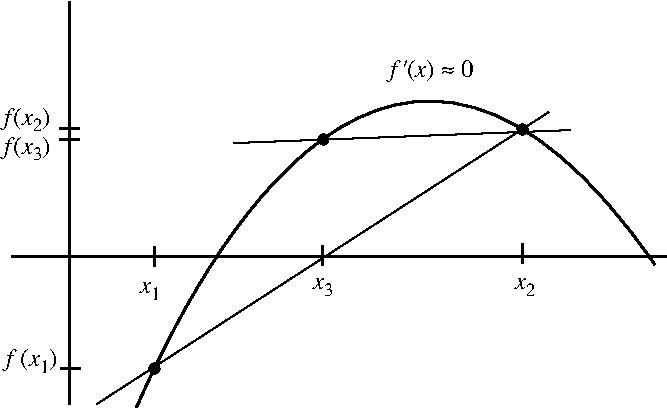
\epsfig{file=eps/secantFails.eps,scale=0.9}}
\end{center}

\vspace{2ex}
Since
\begin{equation*}
    x_{k+1} = x_k - f(x_k) \left[ \frac{x_k - x_{k-1}}{f(x_k) - f(x_{k-1})} \right]
\end{equation*}

the new guess, $x_{k+1}$, will be far from the old guess
whenever $f(x_k)\approx f(x_{k-1})$ and $|f(x)|$ is not small.


% ------------
\end{frame}
%%%%%%%%%%%%%%%%%%%%%%%%%%%%%%%%%%%%%%%%%%%%%%%%%%%%%%%%%%%%%%%%%%%%%%%%
%%%%%%%%%%%%%%%%%%%%%%%%%%%%%%%%%%%%%%%%%%%%%%%%%%%%%%%%%%%%%%%%%%%%%%%%
\begin{frame}
\frametitle{Summary}

\begin{itemize}
\item   Plot $f(x)$ before searching for roots
		\vspace{2ex}
\item   Bracketing finds coarse interval containing roots
		and singularities
		\vspace{2ex}
\item   Bisection is robust, but converges slowly
		\vspace{2ex}
\item   Newton's Method
	\begin{itemize}
		\item   Requires $f(x)$ and $f'(x)$.
		\item   Iterates are not confined to initial bracket.
		\item   Converges rapidly ($r=2$).
		\item   Diverges if $f'(x)\approx 0$ is encountered.
	\end{itemize}
		\vspace{2ex}
\item   Secant Method
	\begin{itemize}
		\item   Uses $f(x)$ values to approximate $f'(x)$.
		\item   Iterates are not confined to initial bracket.
		\item   Converges almost as rapidly as Newton's method ($r\approx
1.62)$.
		\item   Diverges if $f'(x)\approx 0$ is encountered.
	\end{itemize}
\end{itemize}




% ------------
\end{frame}
%%%%%%%%%%%%%%%%%%%%%%%%%%%%%%%%%%%%%%%%%%%%%%%%%%%%%%%%%%%%%%%%%%%%%%%%
\begin{frame}[fragile]
\frametitle{\texttt{fzero} Function}

\texttt{fzero} is a hybrid method that combines bisection,
secant and reverse quadratic interpolation

\vspace{3ex}
\begin{lstlisting}[language=matlab]
r = fzero('fun',x0)
r = fzero('fun',x0,options)
r = fzero('fun',x0,options,arg1,rg2,...)
\end{lstlisting}

\vspace{3ex}
\texttt{x0} can be a scalar or a two element vector
\begin{itemize}
    \item   If \texttt{x0} is a scalar, \texttt{fzero} tries to
            create its own bracket.
    \item   If \texttt{x0} is a two element vector, \texttt{fzero}
            uses the vector as a bracket.
\end{itemize}



% ------------
\end{frame}
%%%%%%%%%%%%%%%%%%%%%%%%%%%%%%%%%%%%%%%%%%%%%%%%%%%%%%%%%%%%%%%%%%%%%%%%
%%%%%%%%%%%%%%%%%%%%%%%%%%%%%%%%%%%%%%%%%%%%%%%%%%%%%%%%%%%%%%%%%%%%%%%%
\begin{frame}
\frametitle{Reverse Quadratic Interpolation}

\vspace{2ex}
Find the point where the $x$ axis intersects the sideways parabola passing
through three pairs of $(x,f(x))$ values.

\begin{center}
	\pgfimage[height=5cm]{./figs/fzeroPicture}
\end{center}

(We'll learn how to do this efficiently in a few lectures.)

% ------------
\end{frame}
%%%%%%%%%%%%%%%%%%%%%%%%%%%%%%%%%%%%%%%%%%%%%%%%%%%%%%%%%%%%%%%%%%%%%%%%
%%%%%%%%%%%%%%%%%%%%%%%%%%%%%%%%%%%%%%%%%%%%%%%%%%%%%%%%%%%%%%%%%%%%%%%%
\begin{frame}
\frametitle{Why (Reverse) Quadratic Interpolation?}
\begin{itemize}
\item If $f(x) = a + bx + cx^2$, and $f(x)$ has real roots, then quadratic 
interpolation gives the answer in one step.
\item Recall that Newtons's method will get the answer in one step
  only if $f(x) = a + bx$.  
\item What if $f(x) = a + bx + cx^2 \ne 0$ for any real $x$?  What
  then?
\item Instead, interpolate the inverse function: $x = g(y) = \alpha +
  \beta y + \gamma y^2$.  If $x = g(y)$, then the root is $x = g(0) =
  \alpha$.
\item What can still go wrong?
\end{itemize}

\end{frame}
%%%%%%%%%%%%%%%%%%%%%%%%%%%%%%%%%%%%%%%%%%%%%%%%%%%%%%%%%%%%%%%%%%%%%%%%
%%%%%%%%%%%%%%%%%%%%%%%%%%%%%%%%%%%%%%%%%%%%%%%%%%%%%%%%%%%%%%%%%%%%%%%%
\begin{frame}
\frametitle{\texttt{fzero} Function}

\texttt{fzero} chooses next root as
\begin{itemize}
    \item   Result of reverse quadratic interpolation (RQI) if that result
            is inside the current bracket.
    \item   Result of secant step if RQI fails, and if the result of secant
            method is in inside the current bracket.
    \item   Result of bisection step if both RQI and secant method fail
            to produce guesses inside the current bracket.
\end{itemize}

% ------------
\end{frame}
%%%%%%%%%%%%%%%%%%%%%%%%%%%%%%%%%%%%%%%%%%%%%%%%%%%%%%%%%%%%%%%%%%%%%%%%
%%%%%%%%%%%%%%%%%%%%%%%%%%%%%%%%%%%%%%%%%%%%%%%%%%%%%%%%%%%%%%%%%%%%%%%%
\begin{frame}[fragile]
\frametitle{\texttt{fzero} Function}

Optional parameters to control \texttt{fzero} are specified with
the \texttt{optimset} function.

\bigskip
Tell \texttt{fzero} to display the results of each step:
\vspace{0.0cm}
\begin{lstlisting}[language=matlab]
>> options = optimset('Display','iter');
>> x = fzero('myFun',x0,options)
\end{lstlisting}

\vspace{3ex}

Tell \texttt{fzero} to use a relative tolerance of $5\times10^{-9}$:
\vspace{0.0cm}
\begin{lstlisting}[language=matlab]
>> options = optimset('TolX',5e-9);
>> x = fzero('myFun',x0,options)
\end{lstlisting}

\vspace{3ex}

Tell \texttt{fzero} to suppress all printed output, and
use a relative tolerance of $5\times10^{-4}$:
\vspace{0.0cm}
\begin{lstlisting}[language=matlab]
>> options = optimset('Display','off','TolX',5e-4);
>> x = fzero('myFun',x0,options)
\end{lstlisting}

% ------------
\end{frame}
%%%%%%%%%%%%%%%%%%%%%%%%%%%%%%%%%%%%%%%%%%%%%%%%%%%%%%%%%%%%%%%%%%%%%%%%
%%%%%%%%%%%%%%%%%%%%%%%%%%%%%%%%%%%%%%%%%%%%%%%%%%%%%%%%%%%%%%%%%%%%%%%%
\begin{frame}[fragile]
\frametitle{\texttt{fzero} Function}

Allowable options (specified via \texttt{optimset}):
\begin{center}
    \renewcommand{\arraystretch}{1.3}
    \small
    \begin{tabular}{llp{12cm}}
        \multicolumn{1}{c}{Option type}
        & \multicolumn{1}{c}{Value}
        & \multicolumn{1}{c}{Effect}  \\
        \hline
        \texttt{'Display'} & \texttt{'iter'}  & Show results of each iteration \\
                           & \texttt{'final'} & Show root and original bracket \\
                           & \texttt{'off'}   & Suppress all print out \\[16pt]
        \texttt{'TolX'}    & \texttt{tol}     & Iterate until\\
                           &                  & \qquad$\displaystyle\left|\Delta x\right|<\max\left[\mathtt{tol},\mathtt{tol}*\mathtt{a}, \mathtt{tol}*\mathtt{b}\right]$\\
                           &                  & where $\Delta x = (b-a)/2$, and $[a,b]$ is the current bracket. \\
         \hline
    \end{tabular}
\end{center}

\vspace{2ex}
The default values of \texttt{'Display'} and \texttt{'TolX'}
are equivalent to
\begin{lstlisting}[language=matlab]
options = optimset('Display','iter','TolX',eps)
\end{lstlisting}

% ------------
\end{frame}
%%%%%%%%%%%%%%%%%%%%%%%%%%%%%%%%%%%%%%%%%%%%%%%%%%%%%%%%%%%%%%%%%%%%%%%%
\begin{frame}[fragile]
\frametitle{\texttt{fzero} example}
Take
\begin{equation*}
  f(x) = x^{10} - 1
\end{equation*}

\vspace{1cm}
\begin{lstlisting}[language=matlab]
>> f = @(x)x.^10 - 1;
>>  options = optimset('display','iter');
>> [x,fx]=fzero(f,0.5,options)
\end{lstlisting}
\end{frame}
%%%%%%%%%%%%%%%%%%%%%%%%%%%%%%%%%%%%%%%%%%%

\end{document}
